\chapter{Clean Architecture}
In diesem Kapitel steht die Clean Architecture und deren zentrale Aspekte im Fokus. Zuerst erfolgt eine Analyse der Dependency Rule, einer Schlüsselregel der Clean Architecture. Untersucht werden dabei die Auswirkungen dieser Regel auf die Softwarearchitektur, ergänzt durch positive und negative Anwendungsbeispiele.

Im Anschluss daran richtet sich der Fokus auf die Struktur der Clean Architecture, wobei die einzelnen Schichten detailliert analysiert werden. Besondere Aufmerksamkeit gilt dabei den Schichten "Domain" und "Application", deren Rolle und Bedeutung innerhalb der Clean Architecture ausführlich diskutiert werden. Diese Analysen ermöglichen ein tiefgreifendes Verständnis der Clean Architecture und ihrer praktischen Anwendung.
\section{Was ist Clean Architecture}
Die \textit{Clean Architecture}, auch bekannt als die \textit{Onion Architecture}, ist ein Software-Entwurfsprinzip, das von Robert C. Martin, entwickelt wurde. Sie zielt darauf ab, eine klare und getrennte Struktur in Software-Systemen zu schaffen, um Wartbarkeit, Testbarkeit und Flexibilität zu verbessern.

Die Clean Architecture teilt eine Anwendung in konzentrische Schichten auf, wobei jede Schicht bestimmte Arten von Aufgaben erfüllt und klar definierte Abhängigkeiten aufweist. Die Schichten, von innen nach außen, sind in der Regel wie folgt:

\begin{figure}[ht]
    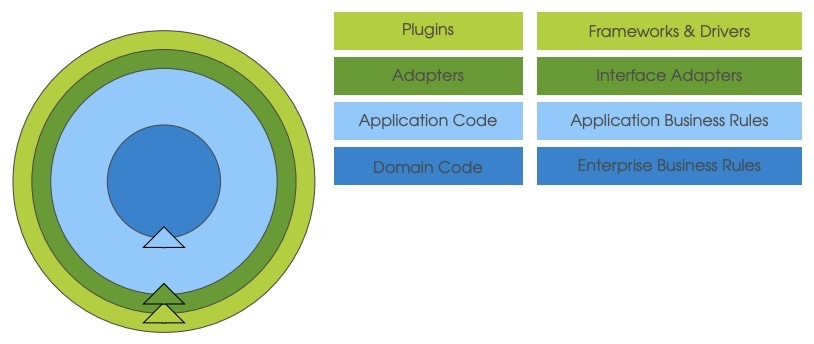
\includegraphics[width=1\textwidth]{Bilder/clean-architecture.jpeg}
    \caption{Clean Architecture Schichten}
    \label{fig:clean-architecture}
\end{figure}
\newpage
\textbf{Domain-Schicht}: Dies ist die innere Schicht, die die Geschäftslogik und die Geschäftsregeln einer Anwendung enthält. Sie hat keine Abhängigkeiten von den äußeren Schichten und repräsentiert die fundamentalen Konzepte der Anwendung, unabhängig von spezifischen technologischen Details.\\

\textbf{Anwendungs-Schicht}: Diese Schicht enthält spezifische Geschäftslogik, die sich auf bestimmte Anwendungsfälle bezieht. Sie ist von der Domain-Schicht abhängig und kann mit ihr interagieren, aber sie kennt keine Details über äußere Schichten.\\

\textbf{Adapter-Schicht}: Diese Schicht übersetzt Daten zwischen den Formaten, die für die inneren Schichten und die äußeren Schichten geeignet sind. Sie könnte beispielsweise Datenbankcode, Benutzeroberflächen-Code oder sogar Code für externe Dienste enthalten.\\

\textbf{Plugin-Schicht}: Dies ist die äußerste Schicht, die spezifische Technologien wie Datenbanken, Webserver oder Frameworks umfasst. Sie interagiert mit den inneren Schichten durch Ports und Adapter.
\newpage
Das Hauptprinzip der Clean Architecture ist die Regel der Abhängigkeitsrichtung: Abhängigkeiten sollten immer von äußeren Schichten zu inneren Schichten gerichtet sein. Dies bedeutet, dass der Code in den inneren Schichten unabhängig von spezifischen Frameworks, Datenbanken oder anderen Technologien ist, was ihn einfacher zu testen und zu warten macht.\\

Zusätzlich wird durch die klare Trennung der Verantwortlichkeiten die Einhaltung des \acf{SRP} und des \acf{OCP} aus den SOLID-Prinzipien erleichtert. Es ermöglicht auch eine bessere Modularität und Austauschbarkeit der Komponenten, da Änderungen in einer Schicht sich nicht auf die anderen Schichten auswirken sollten.

Zusammenfassend lässt sich sagen, dass die Clean Architecture ein Ansatz ist, der darauf abzielt, die Unordnung und Komplexität in Softwareprojekten zu reduzieren, indem klare Grenzen und Regeln für die Struktur und Organisation des Codes vorgegeben werden. Sie ermöglicht es Entwicklern, Systeme zu erstellen, die widerstandsfähig gegenüber technologischen Änderungen sind und die sich im Laufe der Zeit leicht anpassen und erweitern lassen.
\section{Analyse der Dependency Rule}
d
\section{Positiv-Beispiel: Dependency Rule}
\section{Negativ-Beispiel: Dependency Rule}
\section{Analyse der Schichten}
\subsection{Schicht: Domain}
\subsection{Schicht: Application}